\chapter{Flight Planning}
	Now that stable flight has been achieved in the previous chapter, a mission plan can be formulated. The flight strategy will need to consider multiple elements, including the the constraints of a confined environment. In order to successfully navigate, the platform will require sufficient information about it's surroundings. The electronic requirements have been discussed in Section \ref{SECT_ObjectAvoidance}, this chapter will discuss modelling these sensors to simulate 
	
	The first section will discuss modelling this environment. the second section in this chapter will discuss the mathematical modelling of these sensors for the purpose of the simulation. 
	
	\section{Mathematical modelling}
		\subsection{World Creation}
		In order to correctly model the system, a thorough system identification needs to be completed. This entails real world measurements of the chosen platform. The methods and results from these experiments are covered in this section.
	
		\begin{figure}[H]
			\centering
			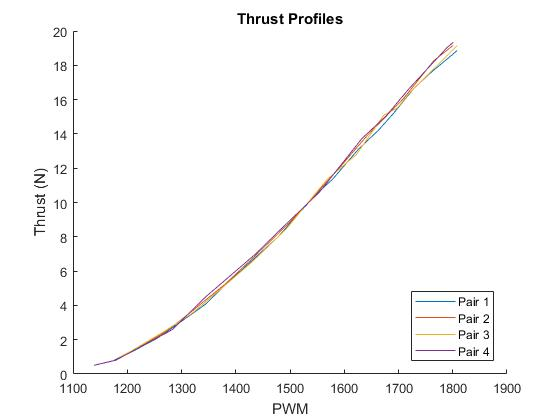
\includegraphics[height = 7.5cm]{../Design/Mechanical/ThrustProfiles/thrustprofiles.jpg}
			\caption{Bifilar Pendulum for Measurement}
			\label{IM_ThrustProfiles}
		\end{figure}
		
		\begin{table}[!]
			\centering
			\begin{tabular}{l | c | c | c |}
				Pair & Max Thrust & Min Thrust\\
				\hline\hline
				$1$ & 18.8558 & 0.7852\\
				$2$ & 19.1489 & 1.1889\\
				$3$ & 19.1434 & 0.9511\\
				$4$ & 19.3369 & 0.5087\\
			\end{tabular}
			\label{TAB_ThrustProfiles}
			\caption{Measured Moments of Inertia}
		\end{table}
	
		\subsection{Sensor Implementation}
		\begin{figure}[H]
			\centering
			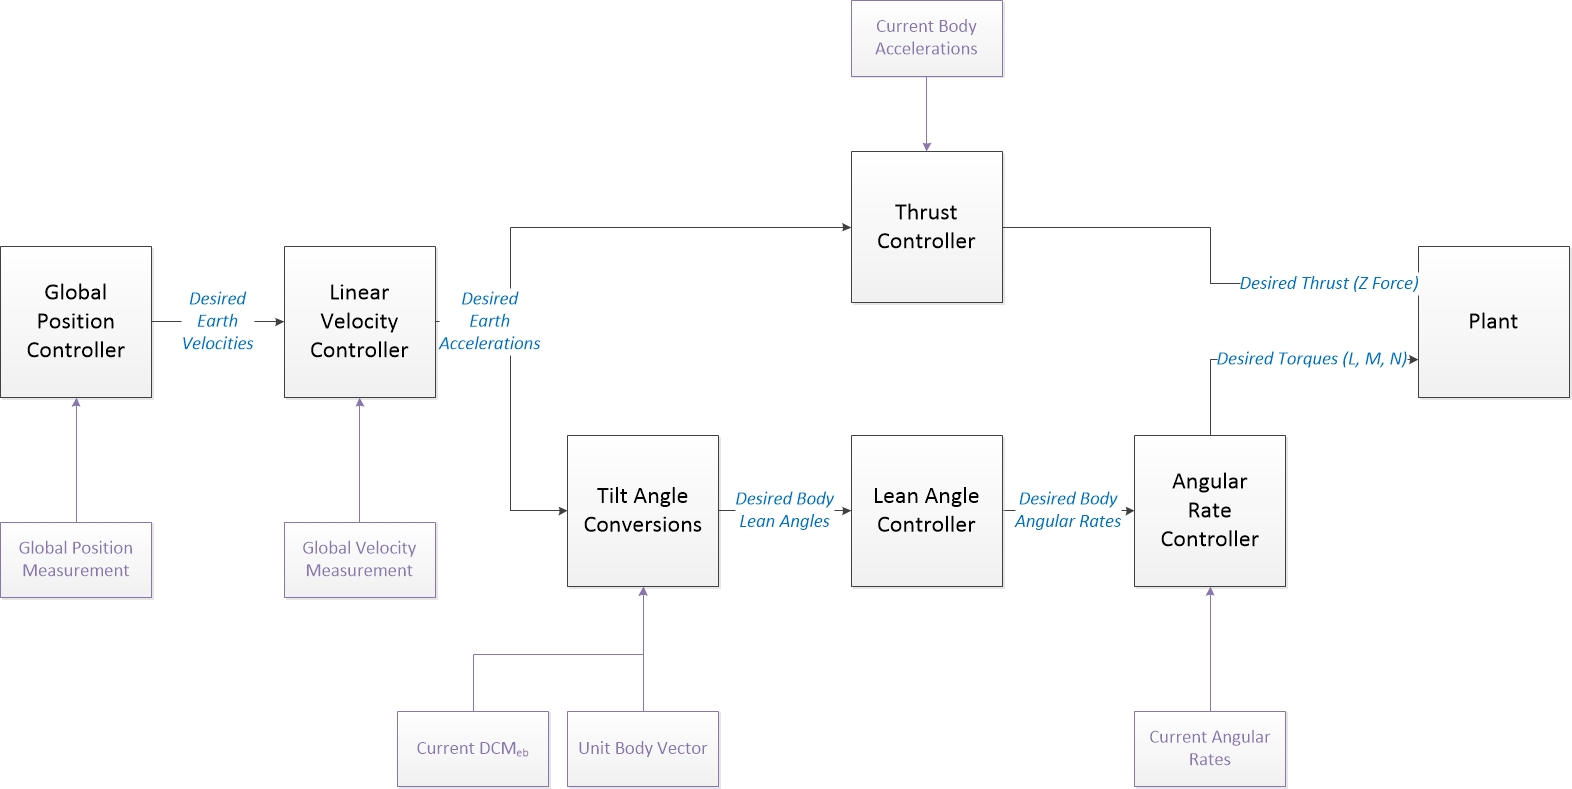
\includegraphics[height = 7.5cm]{../References/Diagrams/ControlDiagram.jpg}
			\caption{High Level Control Strategy}
			\label{IM_ControlStrategy}
		\end{figure}
		
			
		\subsection{Obstacle Avoidance)

	\section{Corridor Flight}
		\subsection{Roll}
		\subsection{Pitch}
		\subsection{Yaw}			
	
	\section{Linear Velocity Control}
